%
%  For more information, please see: http://software.sci.utah.edu
% 
%  The MIT License
% 
%  Copyright (c) 2004 Scientific Computing and Imaging Institute,
%  University of Utah.
% 
%  License for the specific language governing rights and limitations under
%  Permission is hereby granted, free of charge, to any person obtaining a
%  copy of this software and associated documentation files (the "Software"),
%  to deal in the Software without restriction, including without limitation
%  the rights to use, copy, modify, merge, publish, distribute, sublicense,
%  and/or sell copies of the Software, and to permit persons to whom the
%  Software is furnished to do so, subject to the following conditions:
% 
%  The above copyright notice and this permission notice shall be included
%  in all copies or substantial portions of the Software.
% 
%  THE SOFTWARE IS PROVIDED "AS IS", WITHOUT WARRANTY OF ANY KIND, EXPRESS
%  OR IMPLIED, INCLUDING BUT NOT LIMITED TO THE WARRANTIES OF MERCHANTABILITY,
%  FITNESS FOR A PARTICULAR PURPOSE AND NONINFRINGEMENT. IN NO EVENT SHALL
%  THE AUTHORS OR COPYRIGHT HOLDERS BE LIABLE FOR ANY CLAIM, DAMAGES OR OTHER
%  LIABILITY, WHETHER IN AN ACTION OF CONTRACT, TORT OR OTHERWISE, ARISING
%  FROM, OUT OF OR IN CONNECTION WITH THE SOFTWARE OR THE USE OR OTHER
%  DEALINGS IN THE SOFTWARE.
%


\chapter{Working with Networks}
\label{ch:workwithnets}

This section describes how to create, save, load, execute, and edit
networks.

The following conventions are used when describing mouse and keyboard
actions performed by the user:

\begin{description}
\descitem{Button1} Left mouse button

\descitem{Button2} Middle mouse button

\descitem{Button3} Right mouse button

\descitem{Press} ``Press'' means press and hold a key or mouse button.

\descitem{Click} ``Click'' means press and release a mouse button.

\descitem{Type} ``Type''  means press and release a key.

\descitem{Button\replaceable{N}-Drag} Press Button\replaceable{N},
then drag the mouse.

\descitem{C-Button\replaceable{N}} Press the \keyboard{Control} key,
then press or click Button\replaceable{N}

\descitem{C-\replaceable{key}} Press and hold the control key, then
type key \replaceable{key}
\end{description}


\section{Anatomy of a Module}
\label{sec:modanatomy}

%begin{latexonly}
\newcommand{\modgraphic}{%
  \centerline{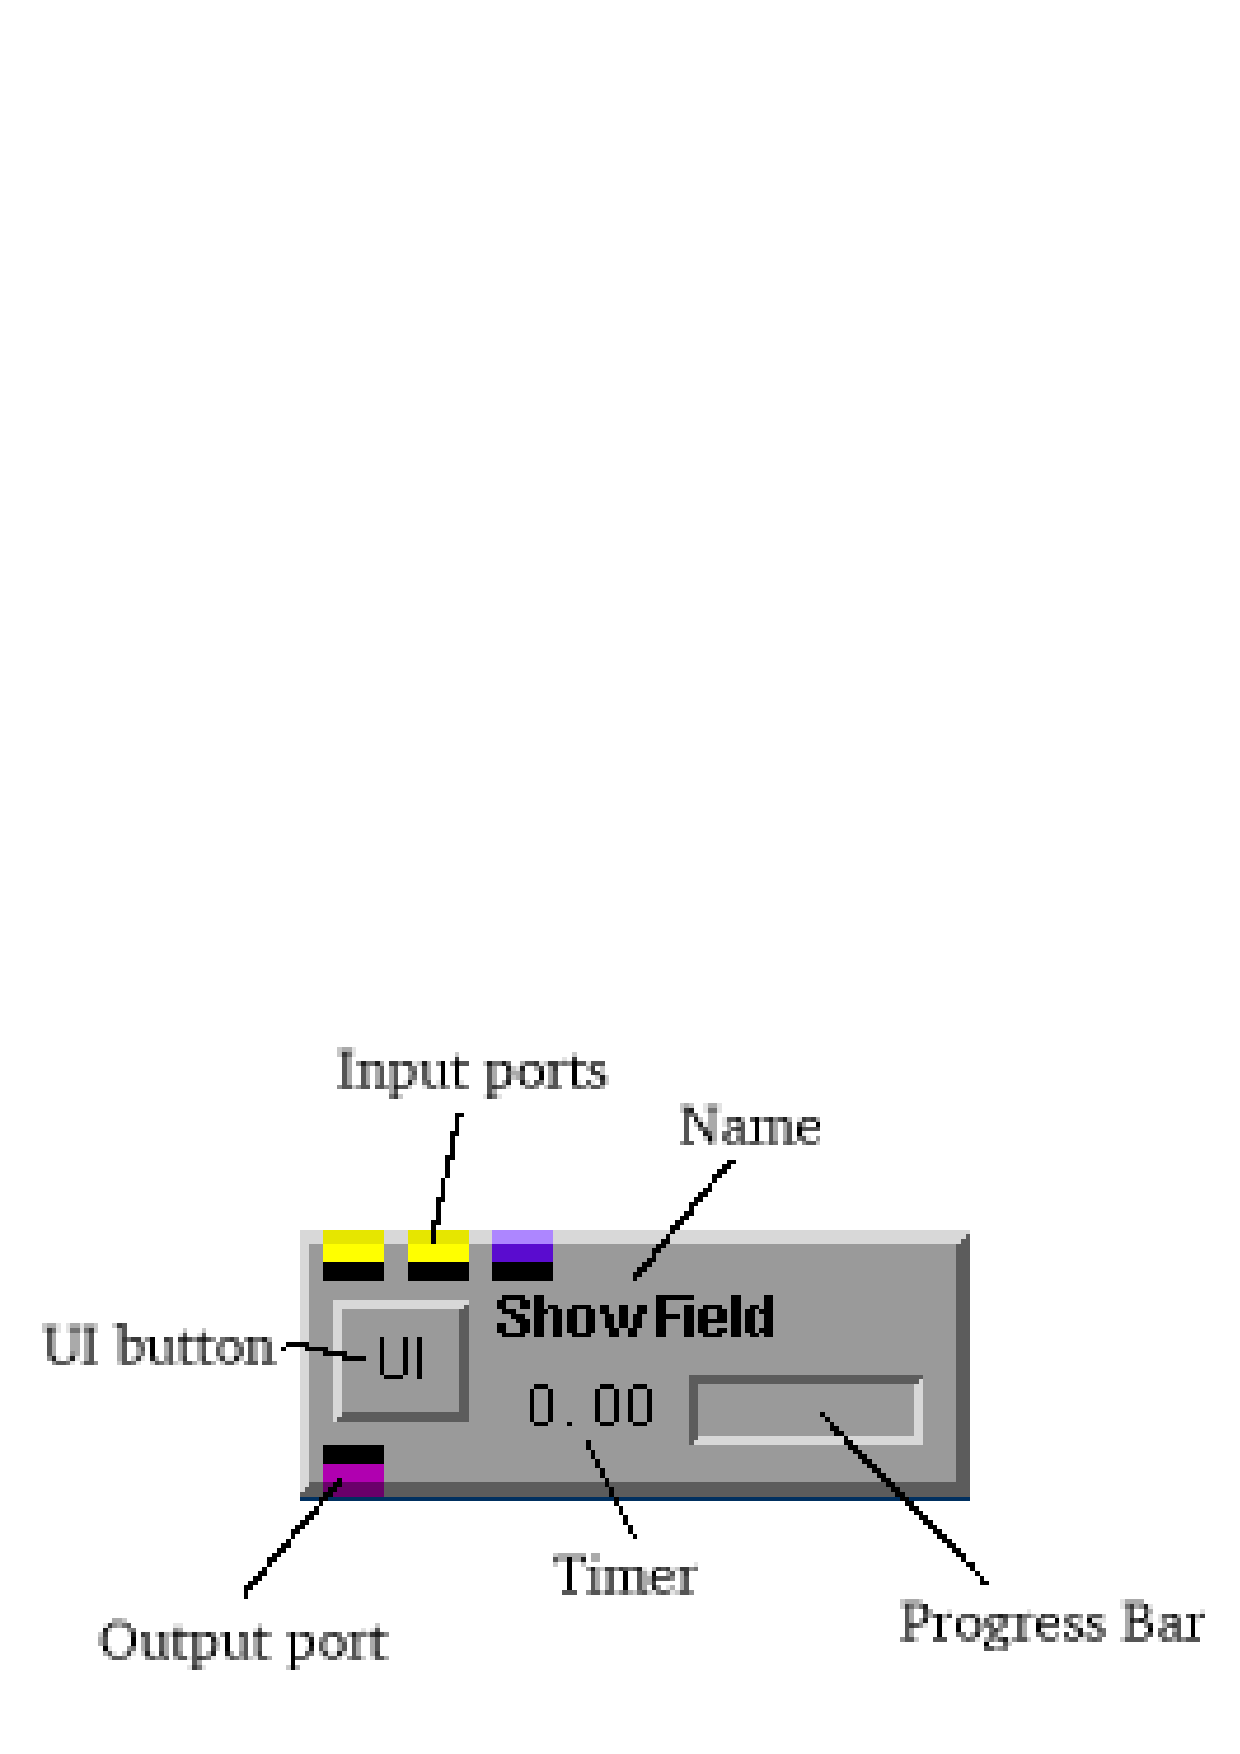
\includegraphics[bb=0 0 325 157,width=4in]{Figures/modgraphic-1.eps.gz}}
}
%end{latexonly}
\begin{htmlonly}
  \newcommand{\modgraphic}{%
  \htmladdimg[alt="SCIRun Module Graphic"]{../Figures/modgraphic-1.gif}
}
\end{htmlonly}

All modules \index{module} are similarly represented by a graphic within the NetEdit frame
(see Figure~\ref{fig:modgraphic}). The graphical ``front end'' is the same
for all modules and consists of the following elements:

\begin{figure}[htb]
  \begin{makeimage}
  \end{makeimage}
  \modgraphic
  \caption{\label{fig:modgraphic} Module Graphic (\module{Show
      Field} Module)}
\end{figure}

\begin{description}
  \descitem{Module Name} The module's name.
  
  \descitem{Input Ports} Zero or more input ports located on the top
  of the module.  Each port corresponds to a data type and each data
  type has a unique color.  Table~\ref{tab:portcolors} maps port
  colors to data types.  Input ports connect to other modules' output
  ports.  Connections can only be made between ports of the same type.
  Some modules have a \dfn{dynamic} input port.  When a connection is
  made to a dynamic input port a new instance of the port will be
  created.

  \begin{table}[htbp]
    \begin{center}
      \begin{tabular}{|l|l|}
        \hline
        \textbf{Data Type} & \textbf{Port Color} \\
        \hline
        Field & Yellow \\
        Field Set & Green \\
        Matrices & Blue \\
        Geometric Objects & Pink \\
        Color Maps & Purple \\
        Camera Path & Brown \\
        \hline
      \end{tabular}
      \caption{Data Types and their Port Colors}
      \label{tab:portcolors}
    \end{center}
  \end{table}
  
  \descitem{Output ports} Zero or more output ports located on the
  bottom of the module.  Output ports connect to other modules' input
  ports.  Every module has  at least one input or one output
  port.
  
  \descitem{UI button} Pressing the \guibutton{UI} button displays the
  module's control dialog. Some modules have no dialog, some have
  simple dialogs, and some have complex dialogs that allow elaborate
  control over the module.  Figure~\ref{fig:moddialog} shows the
  control dialog for \module{Show Field} module.  Most module control
  dialogs (except for read/writer modules) contain the following
  buttons:

  \begin{description}
    \descitem{Close}  Closes the control dialog.

    \descitem{Execute} Executes the module.  This may cause other
    modules in the network to execute or ``fire'' (see
    \secref{Executing a Network}{sec:executenet}).
    
    \descitem{Find} Highlights the module in the NetEdit frame
    that owns the control dialog being edited.

    \descitem{?} Displays a module's help information.

  \end{description}

  Reader/writer module control dialogs contain the following button
  set:

  \begin{description}
    \descitem{Set} Sets the read/writer module's filename value to the
    chosen filename then closes the module's control dialog.  In a
    network with multiple reader/writer modules, \guibutton{Set}
    (rather than \guibutton{Execute}) should be used to establish each
    reader/writer module's filename parameter before executing the
    network.
    
    \descitem{Execute}  Sets the read/writer module's filename value
    to the chosen filename, executes the module (reads file contents
    and sends data downstream), and closes the module's
    control dialog.
    
    \descitem{Cancel} Closes the control dialog without setting the
    module's filename value.
    
    \descitem{Find} Highlights the module in the NetEdit frame
    that owns the control dialog being edited.
    
  \end{description}
  
  \descitem{Progress bar} Shows the module's progress.  As the module
  works toward completion of its task, the progress bar is filled
  with red, then yellow, then green.  When the Progress bar
  is green, the module is done.
  
  \descitem{Timer} Displays the amount of CPU time (seconds) the module has
  consumed.  Located to the left of the progress bar.
  
  \descitem{Message Indicator} Indicates the presence of messages in a
  module's log.  Colors represent message types.  Blue represents
  ``remarks'' (informational messages) and yellow represents
  ``warnings'' (attention is needed).  Click \keyboard{Button1} on the
  indicator to display the module's log.
  
  \descitem{Pop-up Menu} Pressing \keyboard{Button3} while the mouse pointer is
  over a module activates a module's pop-up menu.  The content
  of the pop-up menu changes depending on the state of the NetEdit
  window. The following items are available in the pop-up menu:

  \begin{description}
    \menuitemdesc{Package\_Category\_Name\_Instance} This item is a
    label (not a selectable item).  It provides the module's name and
    the category and package to which the module belongs.
    ``Instance'' is a unique number that distinguishes multiple
    instances of the same module.
    
    \menuitemdesc{Execute} Tells the module to execute (or
    re-execute).  This may cause other modules in the network to
    execute or``fire'' (see \secref{Executing a
      Network}{sec:executenet}).

    \menuitemdesc{Help} Displays the module's help window.
    
    \menuitemdesc{Notes} Displays a module's note pad.  The note pad
    is used to document the purpose of a module in a network.  See
    \secref{Displaying Module Notes}{sec:modnotes}.

    \menuitemdesc{Destroy Selected} Destroys the selected modules.
    See \secref{Destroying Module(s)}{sec:destroymod}.
    
    \menuitemdesc{Destroy} Destroys the module See \secref{Destroying
      Module(s)}{sec:destroymod}.

    \menuitemdesc{Duplicate} Duplicates the module, its input connections,
    and its control dialog state.
    
    \menuitemdesc{Replace With} Replaces the module with the chosen
    one.  \menu{Replace With} is a pop-up menu listing modules that
    accept the same connections as the current module.  The chosen
    module replaces the current module.
    
    \menuitemdesc{Show Log} Displays the module's message log.  Most
    modules write messages to their log during the course of
    their execution (see \secref{Viewing a Module's Log}{sec:viewmodslog}).
    
    \menuitemdesc{Make Sub-Network} Creates a sub-network from
    selected modules.  See \secref{Creating a Sub-Network}{sec:crsubnet}.
    
    \menuitemdesc{Expand Sub-Network} Reverses the action of menu item
    \guimenuitem{Make Sub-Network}.  This menu item is available only in
    a sub-network's pop-up menu.  See \secref{Expanding a
      Sub-Network}{sec:expsubnet}.
    
    \menuitemdesc{Disable} Disables a module (or selected modules).
    See \secref{Disabling/Enabling Modules}{sec:disablemod}.
    
    \menuitemdesc{Enable} Enables a module (or selected modules).  See
    \secref{Disabling/Enabling Modules}{sec:disablemod}.

    \menuitemdesc{Fetch UI} Fetch the module GUI from wherever it happens
    to be on the screen and bring it the mouse, or open the GUI if it is
    not already open. Saves time in tracking down a module GUI.

    \menuitemdesc{Return UI} Return the module GUI to its previous location
    on the screen prior to doing a Fetch UI.

  \end{description}
\end{description}


\section{Anatomy of a Connection}
\label{sec:anatcon}
\index{connections}

A connection lets data flow from one module's output port to (usually) another
module's input port.  Sometimes a connection will connect a module's
output port to its input port.

Connections are colored grey if they are disabled.

Pressing \keyboard{Button3} while the mouse pointer is over a connection
activates a connection's pop-up menu.  The content of the pop-up menu
changes depending on the state of the connection. The following items are
available in the pop-up menu:

\begin{description}
  \menuitemdesc{Delete} Deletes a connection.
  
  \menuitemdesc{Insert Module} Creates and inserts a module ``into'' a
  connection.  \menu{Insert Module} is a pop-up menu listing modules
  that contain at least one input and at least one output port
  matching the connection.  The chosen module is created and then the
  connection is routed into the left-most matching input port and out
  of the left-most matching output port.
  
  \menuitemdesc{Disable (or Enable)} Disables (or enables) a connection.
  
  \menuitemdesc{Notes} Displays a connection's note pad.
\end{description}


\section{Creating a Module}
\label{sec:creatingmodules}

To create a module, select its name from one of the package (\eg{}
\sr) menus' category sub-menus. Package menus are accessed from the
main window's menu bar or from the NetEdit frame's pop-up menu.  The
NetEdit frame's pop-up menu is activated by pressing
\keyboard{Button3} (right mouse button) while the mouse pointer is in
the NetEdit frame (but not over a module or connection).  The pop-up
menu contains a list of category sub-menus from the \sr{} package and
other installed packages.  Each category sub-menu provides access to
modules within the category.

After creating a module, its glyph (or graphic representation---see
Figure~\ref{fig:modgraphic}) is placed in the NetEdit frame.

\section{Setting Module Properties}
\label{sec:setmodprops}

%begin{latexonly}
\newcommand{\moddialog} {%
  \centerline{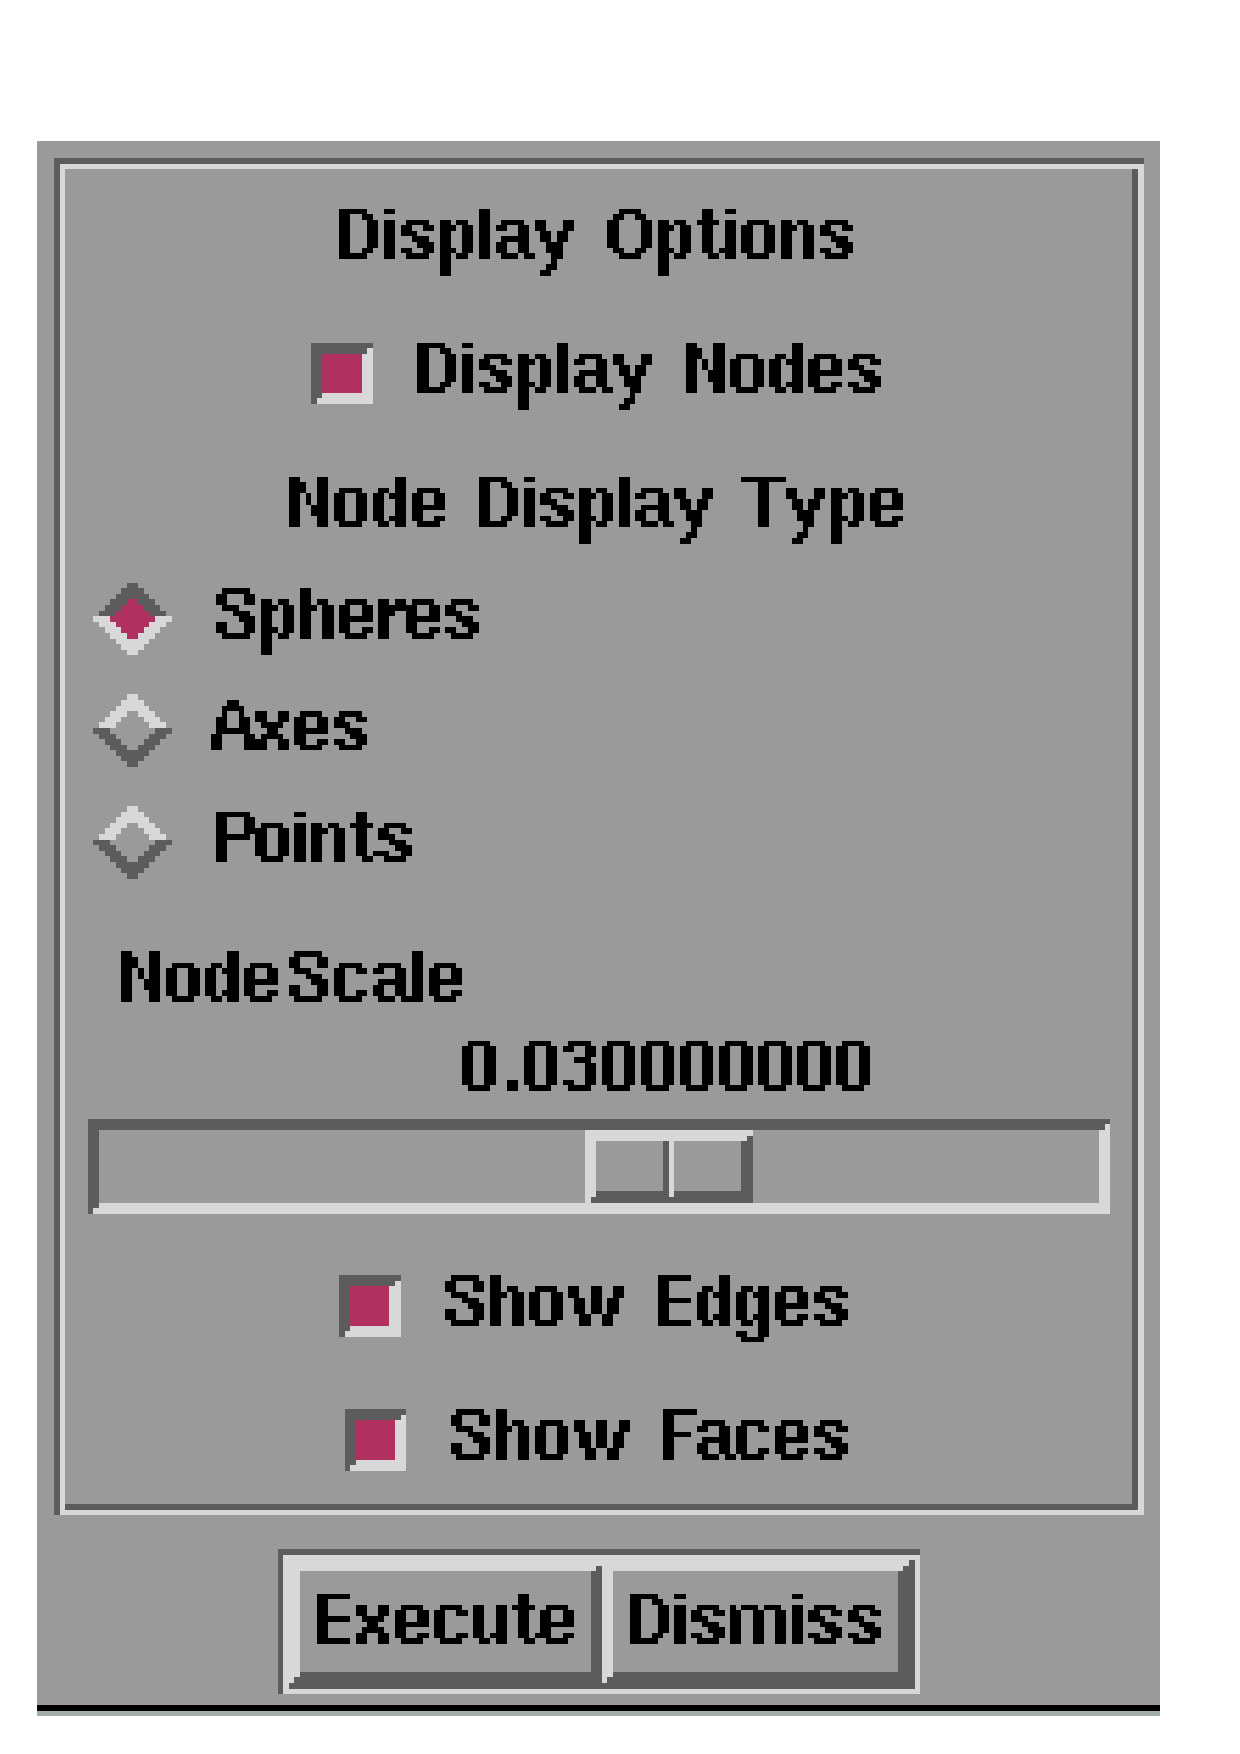
\includegraphics[bb=0 0 275 483]{Figures/moddialog.eps.gz}}
}
%end{latexonly}
\begin{htmlonly}
  \newcommand{\moddialog}{%
    \htmladdimg[alt="SCIRun Module Dialog"]{../Figures/moddialog.gif}
  }
\end{htmlonly}

To change a module's properties, click its \guibutton{UI} button.
This displays the module's control dialog.  Use the dialog to change
the module's properties.  Each \htmladdnormallinkfoot{module's
  reference
  documentation}{\latexhtml{http://software.sci.utah.edu/doc/}{../../../}Developer/Modules/index.html}
explains the use of its control dialog.  A module's reference
documentation can be displayed by clicking a module's \guibutton{?}
button.  Figure~\ref{fig:moddialog} shows the control dialog for the
\module{Show Field} module.

\begin{figure}[htb]
  \begin{makeimage}
  \end{makeimage}
  \moddialog
  \caption{\label{fig:moddialog} Module \module{Show Field}'s Control Dialog
    (User Interface).}
\end{figure}

\section{Selecting Modules}
\label{sec:selectmods}

Some operations (moving, destroying, disabling, and enabling) act on a group of
selected modules (see \secref{Moving Module(s)}{sec:movemod},
\secref{Destroying Module(s)}{sec:destroymod}, and \secref{Disabling  
Modules}{sec:disablemod}).  Groups of selected modules can be created two ways:

\begin{enumerate}
\item Perform \keyboard{Button1-Drag} while the pointer is in the
  NetEdit frame, but not over a module or a connection. This starts a
  selection box, allowing the user to select multiple modules. 
  Modules overlapping the selection box are selected.  Release \keyboard{Button1}
  to complete the selection.  Additional groups of selected modules
  are created by performing \keyboard{C-Button1-Drag}
  
\item Select the first module by clicking \keyboard{Button1} while the
  pointer is over a module.  Then add modules to the group by clicking
  \keyboard{C-Button1} on additional modules.  All previously selected
  modules remain selected.
\end{enumerate}

Selected modules are colored differently from unselected modules.

\section{Destroying Modules}
\label{sec:destroymod}

To delete a module, choose menu item \guimenuitem{Destroy} from a module's
pop-up menu.

Multiple modules can be deleted at one time. Select one or more
modules, then choose menu item \guimenuitem{Destroy Selected} from a
module's pop-up menu.

\section{Moving Modules}
\label{sec:movemod}

Modules can be moved in the NetEdit frame.  To move a module, perform
\keyboard{Button1-Drag} while the pointer is over a module, and move the module
to its new location.

Multiple modules can be moved at one time.  Select one or more
modules, then perform \keyboard{Button1-Drag} while the pointer is over any one
of the modules in the selected group.

Two modules may be moved by dragging one of the connections between
them.  To move two modules, perform \keyboard{Button1-Drag} when the
pointer is over a connection between two modules.

The NetEdit frame will scroll when a module is moved to the frame's edge.

\section{Disabling and Enabling Modules}
\label{sec:disablemod}

Modules may be temporarily disabled.  Disabled modules do not execute
and data does not flow through them.

To disable modules, select one or more modules, then
choose menu item \guimenuitem{Disable} from a module's pop-up menu.

Disabling a module disables all incoming and outgoing connections to
the module and prevents the module from executing during execution of
the network. Disabled modules are drawn in a darker shade of grey.

To enable disabled modules, choose \guimenuitem{Enable} from a disabled
module's pop-up menu.  Enabling one module enables all selected modules.

See also \secref{Disabling/Enabling Connections}{sec:disableconnect}.

\section{Editing and Displaying Module Notes}
\label{sec:modnotes}
\index{annotation of networks}

Module notes allow the user to document the purpose of each module by
attaching notes to each module in the NetEdit window.  Notes can be
displayed or hidden.

To create or edit module notes, choose menu item \guimenuitem{Notes}
from a module's pop-up menu. The note editor dialog can also be
activated by clicking \keyboard{Button1} on notes displayed in the
NetEdit window.  Enter new notes or edit existing notes in the note
editor dialog.

Notes may be hidden, displayed in \dfn{tooltips}, or displayed in the
NetEdit frame.  The note editor provides the following note display
options: \guibutton{Default}, \guibutton{Tooltip}, \guibutton{Top},
\guibutton{Left}, \guibutton{Right}, or \guibutton{Bottom}.  Choose a
display mode by clicking \keyboard{Button1} on the appropriate button.

Choose \guibutton{Tooltip} to display notes as tooltips.  Notes are
displayed only when the mouse pointer hovers over a module.

Choose one of \guibutton{Default}, \guibutton{Top}, \guibutton{Left},
\guibutton{Right}, or \guibutton{Bottom} to display notes in the
NetEdit to the right, top, left, right, or bottom of the module
respectively. 

Choose \guibutton{None} to hide module notes.  Displayed notes can be
hidden by clicking \keyboard{Button2} when the pointer is on the
notes.  Hiding notes does not delete notes.

Click button \guibutton{Text Color} to change the color of notes
displayed in the NetEdit frame.

Click button \guibutton{Cancel} to abort note editing.

Click button \guibutton{Clear} to erase notes.

Click button \guibutton{Done} to accept edited notes.


\section{Viewing a Module's Log}
\label{sec:viewmodslog}

Each module supports a message log. The module writes error messages
or other types of messages to its log.

To display a module's log, choose \guimenuitem{Show Log} from a module's
pop-up menu or click \keyboard{Button1} on a module's message indicator.


\section{Creating a Connection}
\label{sec:connectmods}
\index{connections}

To connect the output (input) port of one module to the input (output)
port of another module, use \keyboard{Button2}.

To make a connection, position the mouse pointer over a module's input
(output) port.  Then perform \keyboard{Button2-Drag} and drag the
mouse pointer toward another module's output (input) port.

When \keyboard{Button2} is pressed, the program shows all valid connections as black
lines.  It also draws one red colored connection, which is the
connection made if the drag is stopped by releasing \keyboard{Button2}.

Make the connection by releasing \keyboard{Button2} when the pointer is over the
desired destination port, or when the red colored connection is the
desired connection.  The connection is drawn using the color
corresponding to the connection's data type.

Users can connect a module's output port to the input ports of one or more
modules by repeating the procedure just described.

\section{Editing and Displaying Connection Notes}
\label{sec:displaynotes}
\index{annotation of networks}

Connection notes allow the user to document the purpose of
each connection by attaching notes to each connection in the NetEdit window.
Notes can be displayed or hidden.

To create or edit connection notes, choose menu item
\guimenuitem{Notes} from a connection's pop-up menu. Enter new notes
or edit existing notes in the note editor dialog.  The note editor
dialog can also be activated by clicking \keyboard{Button1} on notes
displayed in the NetEdit window.

Notes may be hidden, displayed in \dfn{tooltips}, or displayed in the
NetEdit window.  The note editor provides the following note display
options: \guibutton{Default}, \guibutton{Tooltip} and \guibutton{Top}.
Choose a display mode by clicking \keyboard{Button1} on the
appropriate button.

Choose \guibutton{ToolTip} to display notes as tooltips---notes are
displayed only when the mouse pointer hovers over a connection.

Choose \guibutton{Default} or \guibutton{Top} to display notes on top
of the connection.

Choose \guibutton{None} to hide connection notes.  Displayed notes can
also be hidden by clicking \keyboard{Button2} when the pointer is over
the notes.  Hiding notes does not delete notes.

Click button \guibutton{Text Color} to change the color of notes
displayed in the NetEdit frame.

Click button \guibutton{Cancel} to abort note editing.

Click button \guibutton{Clear} to erase notes.

Click button \guibutton{Done} to accept edited notes.


\section{Highlighting Related Connections}
\label{sec:highlightconnect}

To highlight the tree of connections affecting a connection, perform
\keyboard{C-Button1} anywhere on a connection.

To highlight the tree of connections downstream an output port,
perform \keyboard{C-Button1} on the output port.

To highlight the tree of connections upstream an input port,
perform \keyboard{C-Button1} on the input port.

\section{Disabling a Connection}
\label{sec:disableconnect}

To disable a connection, click \keyboard{Button3} on the connection to
bring up the connection menu and select \guimenuitem{Disable}. The
connection appears grey.

Disabling a connection prevents data from flowing through, as if it were
not connected.

\section{Deleting a Connection}
\label{sec:deleteconnections}

To delete a connection, choose menu item \guimenuitem{Delete} from a
connection's pop-up menu or click \keyboard{C-Button2} while the
pointer is on a connection.

\section{Undoing/Redoing a Connection}
\label{sec:undomod}

Type \keyboard{C-z} to undo the last connection creation or deletion.
Undo can be repeated.

Type \keyboard{C-y} to redo the last undone connection creation or
deletion.

\section{Executing a Network}
\label{sec:executenet}

``Network Execution'' means one or more modules must be executed in a
coordinated fashion. 
\sr{}'s \dfn{scheduler} manages the coordinated execution of modules.

Note that some modules need to be compiled before they are
executed (see \secref{Dynamic Compilation}{sec:dyncomp}).  Compilation
delays network execution.  Usually, occurs only one time
per module.  After a module is compiled, it does not need to be
compiled again.  Modules change color during compilation.

\subsection{The Basics}

The scheduler is invoked when an event \dfn{triggers} a
module's execution.  The scheduler creates a list of all modules that
must execute in coordination with the triggered module. Modules
\dfn{upstream} (directly or indirectly) from the triggered module are 
put on the execution list if they have not previously executed.
All modules \dfn{downstream} from the triggered module are put
on the execution list.  Once the scheduler determines which modules must be
executed, it executes them (in parallel where possible).

Network execution is mostly transparent.  That is, events that trigger
module execution usually generate automatically. Sometimes,
however, the user must manually
generate a triggering event by choosing the \guimenuitem{Execute} item from a
module's pop-up menu.

\subsection{Details}

Each module executes in its own thread and blocks (waits) until its upstream
modules can supply it with data.  After a module completes its computation,
it sends the results to its downstream modules.  This completes a module's
execution cycle.  The module will not have another chance to receive data from its input ports
and send data to its output ports until some event
puts the  module back on the scheduler's execution list.  

This behavior prevents modules from computing in an iterative fashion 
(sending intermediate results to their downstream modules), because
downstream modules cannot receive results until they are in their
execution cycle. Downstream modules would need to be executed each time the
upstream module posts an intermediate result.


\subsection{Intermediate Results}

Some modules are designed to be used in an iterative fashion. They use
a method called \icode{send\_intermediate} to send the results of each
iteration.  When this method is used, the scheduler (re)executes
downstream modules each time the upstream module posts its next
result.  Downstream modules are able to receive the results of each
iteration as soon as the upstream module sends them.

Modules \module{SolveMatrix} and \module{MatrixSelectVector} (from the
\package{\sr} package and \category{Math} category) are examples of modules
that compute iteratively using the \icode{send\_intermediate} method.

\subsection{Feedback Loops}

Some modules are designed to be used exclusively in feedback
loops. Their output ports can be connected
directly or indirectly to their input ports.  These modules also use the
\icode{send\_intermediate} method.

Examples of feedback modules are \module{DipoleSearch} and
\module{ConductivitySearch} from the \category{Inverse} category of the
\package{BioPSE} package and \module{BuildElemLeadField} from the
\category{LeadField} category of the \package{BioPSE} package.

\section{Documenting a Network}
\label{sec:docnetwork}
\index{annotation of networks}

It is useful to document the function of a network.  A network's note
pad is used for this purpose.  To edit the network's note pad,
select the \guimenuitem{Add Info} item from the main window's \menu{File}
menu.  This displays the network's note pad editor.  The editor
allows the user to write notes on the purpose and use of the network.

\section{Saving a Network}
\label{sec:savenet}

\sr{} can save networks to files.  Network files have an extension of
\filename{.net} (in the past they also had .sr and .uin
extensions).  

To save a network, select item \guimenuitem{Save} from the main window's
\menu{File} menu.  A file browser dialog prompts for the
name and location of the network file.

If changes are made to an existing network, \guimenuitem{Save} saves
changes made to an existing net file.

Save an existing network under a new name using the \guimenuitem{Save
  As...} menu item.  A file browser dialog prompts for the new name of
the network file.  Subsequent uses of \guimenuitem{Save} saves changes
to the newly created file.

The position and size of open Viewer windows are saved to
the network file.

Network files are  \dfna{Tool Command Language}{TCL} scripts.
These files can be edited, however, reasons for doing so are beyond
the scope of this guide.

\section{Loading a Network}
\label{sec:opennet}

To load a network file, select the \guimenuitem{Load} item from the main
window's \menu{File} menu.   A file browser dialog prompts for the
name and location of the network file.  The loaded network replaces an
existing network in the NetEdit frame.

\section{Inserting a Network}
\label{sec:insertnetwork}

To avoid merging networks, select the
\guimenuitem{Insert} item from the main window's \menu{File} menu. This
option allows the user to place one \sr{} network next to another,
avoiding overlap.  A file browser dialog prompts the user for the name and
location of the network file.

The new network is inserted into the upper left corner of the
NetEdit frame.  If a network of modules already exists in the NetEdit
frame, the \guimenuitem{Insert} command places a new network to the
immediate right of the existing network.

\section{Clearing a Network}
\label{sec:clearnetwork}

To remove all modules and connections from the 
NetEdit frame, select the \guimenuitem{Clear} item from the main window's
\menu{File} menu.  A text box appears, confirming whether the
user wants to proceed with or cancel the clearing operation.

\section{Navigating a Network}
\label{sec:navnetwork}

A complex network may not be entirely visible in the NetEdit frame.
Use the NetEdit frame's scroll bars or the network view tool to view
complex networks.

The Global View Frame \index{global view frame}shows the 
entire ``network world.''  The small
rectangular region (outlined in black) in the Global View Frame is the
network view tool and a window on the network world. The position of
the view tool determines the part of the network visible in the
NetEdit frame.  To view other parts of the network, press
\keyboard{Button1} while the pointer is anywhere in the Global View
Frame---this moves the tool to the location of the pointer -- then
drag the tool to the new location.

\section{Creating a Sub-Network}
\label{sec:crsubnet}
\index{sub-network}

%begin{latexonly}
\newcommand{\subnetgraphicfig}{%
  \centerline{\includegraphics[bb=0 0 252 144]{Figures/subnetgraphic.eps.gz}}
}
%end{latexonly}
\begin{htmlonly}
  \newcommand{\subnetgraphicfig}{%
    \htmladdimg[alt="Graphic of a Sub-network"]{../Figures/subnetgraphic.gif}
  }
\end{htmlonly}


A sub-network is a group of modules that are treated as a single
module.  In a network, you may use a sub-network as you would a
module.

To create a sub-network, select one or more modules, then choose item
\guimenuitem{Create Sub-Network} from any selected module's pop-up menu.
Selected modules will be replaced by a sub-network graphic and the
sub-network editor will activate.  Sub-networks may be created in
sub-networks.  The next section (\secref{Editing a
  Sub-Network}{sec:editsubnet}) explains the use of the sub-network
editor.

A sub-network editor button replaces the CPU time and Progress
Bar in the sub-network graphic.  See Figure~\ref{fig:subnetgraphic}

\begin{figure}[htb]
  \centering
  \begin{makeimage} \end{makeimage}
  \subnetgraphicfig
  \caption{\label{fig:subnetgraphic} A Sub-Network in the NetEdit frame}
\end{figure}

A sub-network's editor is activated by pressing the
sub-network editor button.

Pressing button \guibutton{UI} activates control dialogs of all
modules in a sub-network.  Control dialogs can be activated
individually in the sub-network editor.

In a network, a sub-network behaves as does a module.  A sub-network
has input and/or output ports (orginating from modules within the
sub-network) that can be connected to modules outside of the
sub-network.  Each sub-network has a pop-up menu and a set of editable
notes (see \secref{Editing and Displaying Module
  Notes}{sec:modnotes}).  A sub-network does not have a log. Logs of
individual modules in the sub-network can be viewed in the sub-network
editor window (see \secref{Viewing a Module's Log}{sec:viewmodslog}).

\section{Expanding a Sub-Network}
\label{sec:expsubnet}

Expanding a network reverses the action of menu item \guimenuitem{Create
  Sub-Network}---all modules in a sub-network are returned to the
network containing the sub-network and the sub-network is destroyed.
This action cannot be undone.

To expand a sub-network choose menu item \guimenuitem{Expand Sub-Network}
from the sub-network's pop-up menu.

\section{Editing a Sub-Network}
\label{sec:editsubnet}

%begin{latexonly}
\newcommand{\subneteditorfig}{%
  \centerline{\includegraphics[bb=0 0 304 307]{Figures/subneteditor.eps.gz}}
}
%end{latexonly}
\begin{htmlonly}
  \newcommand{\subneteditorfig}{%
    \htmladdimg[alt="Sub-net editor"]{../Figures/subneteditor.gif}
  }
\end{htmlonly}

The sub-network editor is activated by pressing a sub-network's editor
button.  The sub-network editor works similarly to the NetEdit window.
All network editing features of the NetEdit window are available in
the sub-network editor---modules can be created, connections can be
made, \etc{} See Figure~\ref{fig:subneteditor}.

\begin{figure}[htb]
  \centering
  \begin{makeimage} \end{makeimage}
  \subneteditorfig
  \caption{\label{fig:subneteditor} Sub-network editor.}
\end{figure}

Sub-networks have input and/or output ports.  These are created in the
sub-network editor.  Sub-network input ports are created by making a
connection between the input port of a module (in the sub-network) and
the top edge of the sub-network editor window.  Sub-network output
ports are created by making a connection between the output port of a
module (in the sub-network) and the bottom edge of the sub-network
editor window.

A sub-network can be renamed by entering its new name into the
\guilabel{Name} text entry widget.

\section{Saving a Sub-network}
\label{sec:savesubnet}

Sub-networks can be saved for reuse in networks and sub-networks.

Sub-networks are saved in directory \directory{SCIRun/Subnets}, in the
user's home directory.

To save a sub-network, press the sub-network's editor
button, which activates the sub-network's editor, then press the
editor's \guibutton{Save} button.

Saved sub-networks are listed as menu items in the \menu{Sub-network}
package menu (which is available in the NetEdit window's \menu{File}
menu and popup menu).

\secref{Loading a Sub-Network}{sec:loadsubnet} gives instructions for
loading sub-networks into networks and sub-networks.

%% Note:  I don't like the terminology used here.  ``creating''
%% subnetworks and ``loading'' subnetworks ought to be ``making'' or
%% ``building'' and ``loading'' ought to be ``instantiating'' or
%% ``creating''.
\section{Loading a Sub-Network}
\label{sec:loadsubnet}

Saved sub-networks are loaded into networks and sub-networks by
selecting their names from the \menu{Sub-network} package menu.
Package menus are accessed from the main window's menu bar or from the
NetEdit frame's pop-up menu.  Unlike other package menus, the
\menu{Sub-network} menu has no category sub-menus.

A sub-network may be loaded one or more times in a network.  Each time
a sub-network is loaded a new instance of it is created in the
network.

\section{The \sr{} Shell}
\label{sec:termapp}

After starting, \sr{} runs a shell-like application in the terminal
window. This shell displays the prompt
\screen{scirun\ra} in the terminal window.This program is a
\dfna{Tool Command Language}{TCL} shell program extended with
\sr{} specific commands.

It is possible to type \tcl{} \sr{} commands at the prompt.  For
instance, to load a network type \keyboard{source 
\ptext{network file name}}.  This has the same effect as the \menu{File}
menu's \guimenuitem{Load} command.
